\section{Background and Related Work}\label{sec:background}

%% In this section, we introduce the concepts and terminology that are necessary to understand the reminder of this paper. First, Section~\ref{sec:sand} introduces some background information about \emph{sandboxes} within the security context. Section~\ref{sec:repackage} presents background information about repackaged application and how they introduce malicious behavior.
%% Finally, in Section~\ref{sec:android-sandbox} we review the \emph{mining sandbox approach} for detecting repackaged Android apps.

The Android bytecode language~\cite{DBLP:conf/issta/WangGMC15} favors reverse engineer tasks. That is, software developers can easily reverse-engineer real apps (benign), modify their contents by inserting malicious code (malware), repackage them with the malicious payloads, and re-advertise them in the official market, Google Play Store, or other markets. Repackage Android apps can leverage the popularity of real apps, to increase its propagation and spread malware.  
Repackaging has been raised as a great security problem in Android ecosystem by stakeholders in the app development industry and researchers. There are works~\cite{DBLP:conf/sigmetrics/ViennotGN14} claiming that about 25\% of Google Play Store app content is repackaging apps. Nevertheless, all the workload to detect and remove malware from markets by the stores (official and no official), have not been accurate enough to address the problem as fast as possible. As a result, repackaged Android apps follow threatening security and privacy of unsuspicious Android app users, beyond compromising the copyright of the original developer~\cite{DBLP:journals/access/KimLCP19}. Aiming at
mitigating this threat, static and dynamic analysis approaches have been proposed.

\subsection{Dynamic and Static Analysis on Android apps}\label{sec:analysis}

There is a large body of work that explores the use of program analysis techniques to detect malware. 

Several works have been proposed to detect malware based on sensitive method calls and permission control~\cite{DBLP:conf/mobicom/WeiGNF12,DBLP:conf/asiajcis/WuMWLW12,DBLP:conf/sp/LiDLDG21}. Cai et al.~\cite{DBLP:journals/tse/CaiR21} presented a longitudinal study on Android apps focusing on run-time behaviors. However, this work does not focus specifically on malware detection but on general security gaps in apps by considering only benign apps. Fangfang et al.~\cite{DBLP:conf/wisec/ZhangHZW014} proposed ViewDroid, which models the UIs of Android apps as a directed graph. Although ViewDroid also works by comparing app pairs to identify repackaged apps, their focus is UI centric.

On static analysis approaches exploring Android Manifest files, Kim et al. proposed RomaDroid~\cite{DBLP:journals/access/KimLCP19}.  Their approach does not consider the structural context in Manifest files, but rather treat the files as sequence of strings and perform a lowest common subsequence (LCS) based approach to detect repackaged apps. Au el al.~\cite{DBLP:conf/ccs/AuZHL12} also apply static analysis on Android Manifest files to detect vulnerabilities in Android apps. They do this by mapping requested permissions to sensitive API calls in the code.

Li et al.~\cite{DBLP:journals/tifs/0029LBKTLC17} provided a systematic knowledge on Android malware by conducting an empirical study comparing malicious repackage app with their benign counterparts (1,497 app pairs). They found that the majority of Android malware are repackaged versions of benign apps that donot do anything complex modifications, many times simply reusing library code.

In the domain of detecting repackaged apps by comparing app pairs, Crussell et al.~\cite{DBLP:conf/esorics/CrussellGC12} proposed  DNADroid, which compares program dependence graphs, and Zhou et al.~\cite{DBLP:conf/codaspy/ZhouZJN12} DroidMoss which detects and analyzes repackaged apps using a fuzzy hashing technique. 

\subsection{Mining Android Sandboxes}\label{sec:android-sandbox}

A \emph{sandbox}
is a well-known mechanism to secure a system and forbid a software component to access
resources that it is not allowed to. Sandboxes have also been used to build an isolated
environment on an electronic device within which applications cannot affect other programs, the network, or other device data~\cite{DBLP:journals/peerj-cs/MaassSCS16}. In this scenario, the idea of using sandboxes emerged from the
need to testing unsafe software, possible malware, without worrying about the integrity of the
device under test~\cite{DBLP:conf/esorics/BordoniCS17}, shielding the operation system from any security issue.
To ensure safety, a sandbox environment should have the minimum requirements to run the
program (make sure the program will not escape the sandbox), and make sure it will never
assign the program greater privileges than it should have, working with the principle of
\emph{least privilege}. This principle ensures unauthorized access to resources,
improving the system's overall health. Regarding Android ecosystem, the principle
of the \emph{least privilege} is ensured by sandboxing too,
where apps never access direct resources or data of other apps. Access to sensitives resources
like contacts list is granted through specific APIs (Application Programming Interface),
which are managed by permissions~\cite{DBLP:journals/corr/abs-2109-06613}. 

%% The main market source for Android apps is Google Play Store. Unfortunately, it has
%% a flexible policy regarding the process of publishing apps, and therefore, many Android apps are removed from the
%% store because of issues related to malware\cite{DBLP:conf/msr/WangLL0X18}. Google Play tries
%% to minimize unauthorized access to sensitive resources by malicious apps,
%% listing each app with its requested permission. {\color{red}Those permissions are presented to Android
%% users at app installation moment since version 6}. However, some works presented that most users are careless regarding these permissions since they are only interested to run the app~\cite{DBLP:conf/soups/FeltHEHCW12}. This represents a great security breach since malware usually asks for more permissions than their APIs normally would require~\cite{DBLP:conf/ccs/FeltCHSW11}.



The Mining Android Sandbox approach~\cite{DBLP:conf/icse/JamrozikSZ16} aims at automatically
building a sandbox from dynamic analysis (i.e., using automatic test generation tools).
The main idea is to explore apps based on their calls to sensitive APIs.
Thus, sandboxes build upon these calls to create safety rules and then block future
calls to other sensitive resources, which diverge from those found in the first exploratory
phase. Using a test generation tool named Droidmate~\cite{DBLP:conf/icse/JamrozikZ16},
Jamrozik et al.~\cite{DBLP:conf/icse/JamrozikSZ16} proposed the first mainstream
implementation of the Mining Android Sandbox approach, called Boxmate. 
Boxmate records the occurrences of calls to sensitive APIs and the event that triggers these calls,
like a button click. It is possible to configure Boxmate to record events associated with each sensitive call as
tuples (event, API). Jamrozik et al. argue that, in this way, Boxmate generates finer granularity results which
might reduce false alarms, even with the presence of reflection which is quite commonly used in
malicious apps~\cite{DBLP:conf/issta/0029BOK16}. 

Figure~\ref{fig:mineSandbox} extracted from paper~\cite{DBLP:conf/wcre/BaoLL18}, summarises the approach. 

\begin{figure}[ht]
\centering
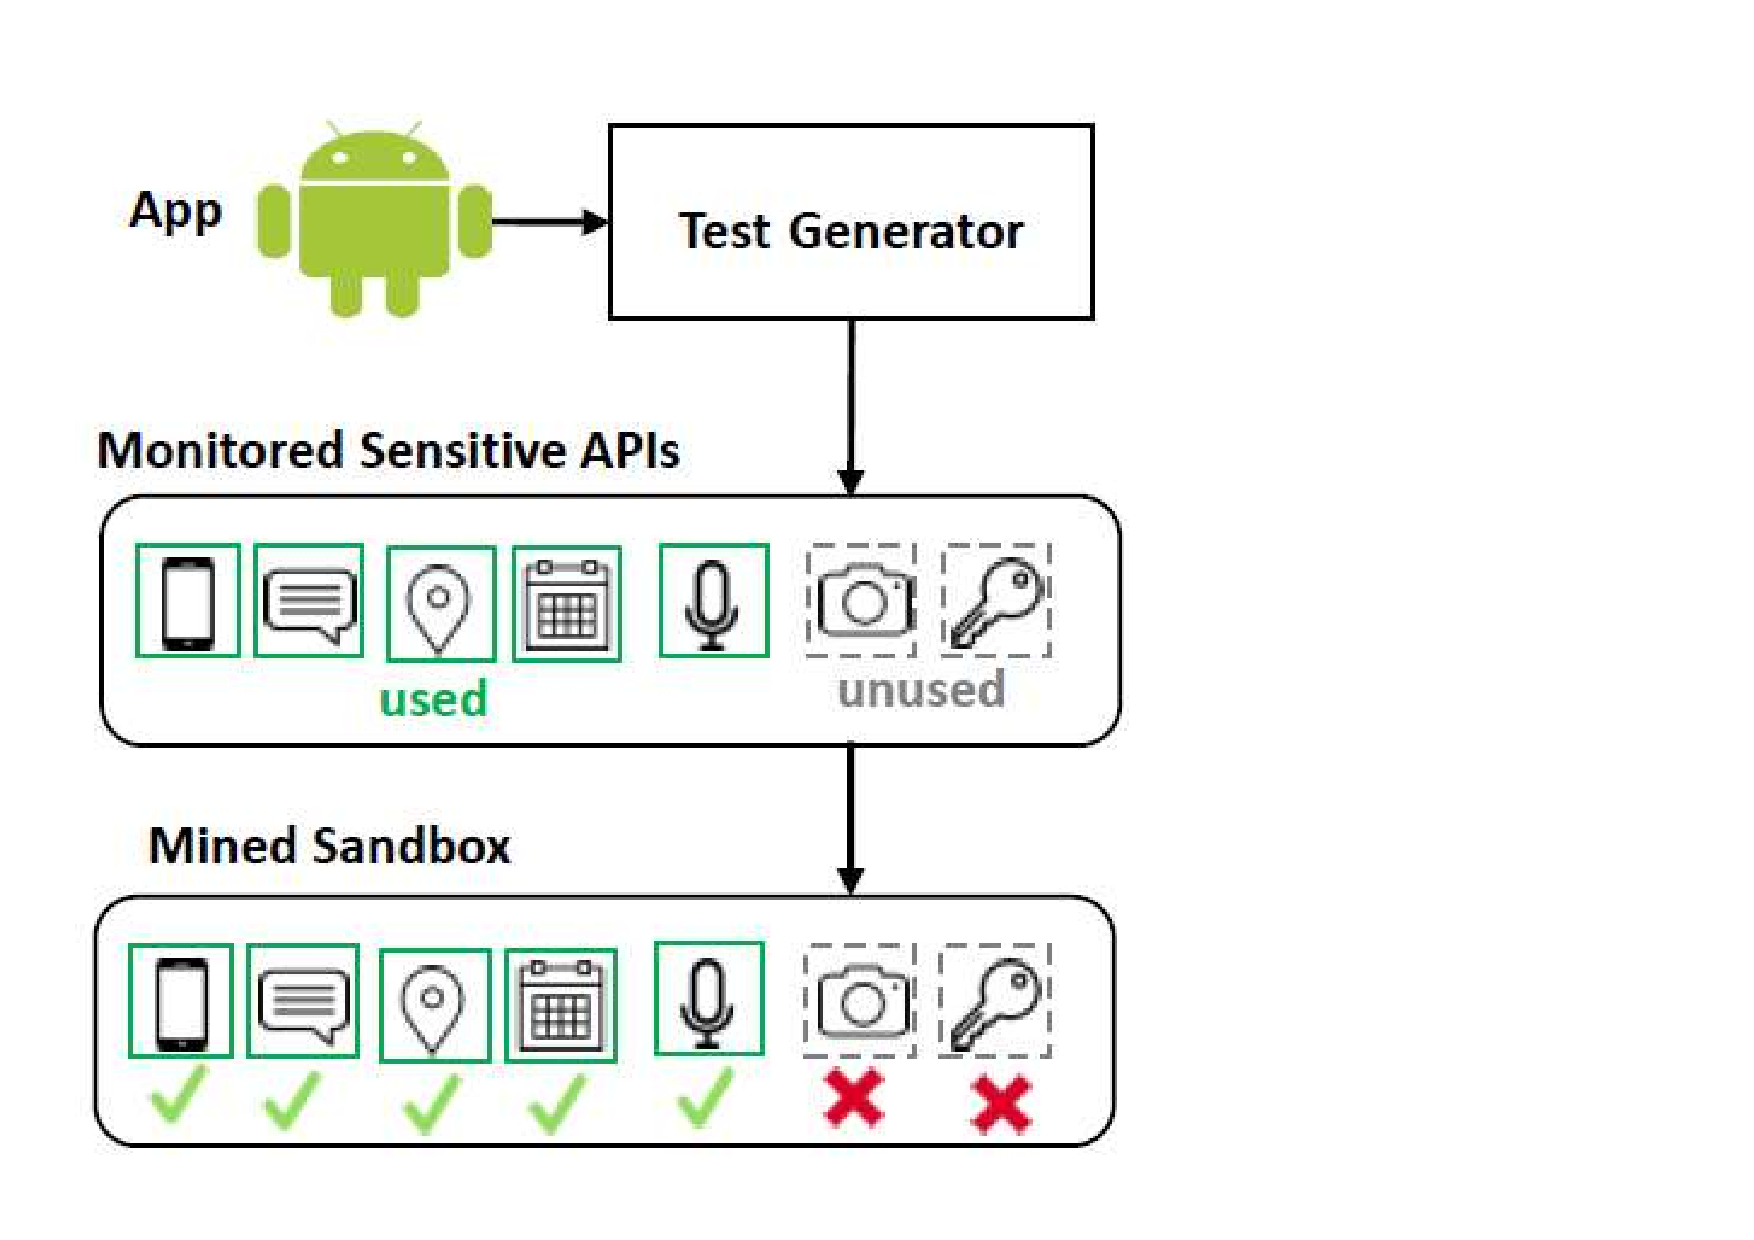
\includegraphics[scale=0.30]{images/mineSandbox.pdf}
\caption{Mine Sandbox. Extracted from~\cite{DBLP:conf/wcre/BaoLL18}}
 \label{fig:mineSandbox}
\end{figure}

The Mining Android Sandbox approach accuracy suggests a close relationship with the
efficiency of the exploratory phase. The more efficient the test generator
tools (for instance, in terms of code coverage), the more accurate would be the resulting
sandbox. Besides being used to generate Android sandboxes, the Mining Android Sandbox approach is also effective 
to classify malwares~\cite{DBLP:conf/wcre/BaoLL18}.  In this scenario, the \emph{effectiveness} of the approach
is estimated in terms of repackage/malware identification.
Previous studies~\cite{DBLP:conf/wcre/BaoLL18,DBLP:conf/scam/CostaMCMVBC20} that explored the effectiveness of mine sandboxes,
investigating and comparing the performance of different test generator tools,
with diverse exploratory strategies.


The focus of our paper is in approaches that mine android sandboxes to detect Android Malware.
There is a vast body of research in this direction. 
Bao et al.~\cite{DBLP:conf/wcre/BaoLL18} conducted an empirical study to investigate the effectiveness of android sandbox approaches
for detecting malware, exploring test generation tools, including Droidmate. The authors found that in general, the sandboxes constructed by test generator tools can detect more than $70$\% malicious apps in a dataset comprising $102$ pairs (benign/malicious). The study also presented that among 5 test generation tools used, DroidBot~\cite{DBLP:conf/icse/LiYGC17} leads to the most efficient sandbox.
Le et al.~\cite{le2018towards} extend the work of Bao et al. by combining more categories of APIs, and also considering the impact of
actual arguments on the sandboxe definition.
None of the aforementioned studies ~\cite{DBLP:conf/icse/JamrozikSZ16,DBLP:conf/wcre/BaoLL18,le2018towards} neither characterize the APIs included on the repackage versions nor investigate the possibility that trace analysis using call graph or analysis of the manifest file could complement the mining sandbox approach for malware identification.

Hence, our work, although closely related to previous studies, differs from them in several aspects. We present a broader assessment of the effectiveness of the mining sandbox approach for malware identification, resulting in the first in depth characterization of the calls to sensitive APIs that frequently appear in the repackage version of the apps. Our assessment is also more comprehensinve: instead of considering $102$ pairs of benign/malign apps, we execute our study consider {\color{red}800} pairs of apps. We also explore two possible strategis to complement the mining sandbox approach for malware identification. The first explores the impact of dynamic call graphs through the comparisons of traces from entry point to the calls to sensitive APIs that result from the executions of the benign and malign versions of an app. The second explores suspicious change patterns in the Android Manifest file of the apps, using a simple, yet effective, static analysis approach.
